\documentclass[a4paper,12pt]{article}

%% Language and font encodings
\usepackage[english]{babel}
\usepackage[utf8]{inputenc}
\usepackage[T1]{fontenc}

%% Page size and margins
\usepackage[a4paper,top=2.5cm,bottom=2.5cm,left=3cm,right=3cm,marginparwidth=1.75cm]{geometry}

%% Core packages
\usepackage{amsmath}
\usepackage{amssymb}
\usepackage{graphicx}
\usepackage{tabularx}
\usepackage{booktabs}
\usepackage{float}
\usepackage{subcaption}
\usepackage[protrusion=true,expansion=false]{microtype}
\usepackage{xcolor}
\usepackage{enumitem}
\usepackage{array}
\usepackage{multirow}
\usepackage{longtable}
\definecolor{tcdBlue}{RGB}{5, 105, 185}
\definecolor{lightgray}{RGB}{245,245,245}

%% Code listings
\usepackage{listings}
\lstset{basicstyle=\small\ttfamily, backgroundcolor=\color{lightgray},
        frame=single, breaklines=true}

%% Hyperlinks
\usepackage[colorlinks=true,linkcolor=tcdBlue,citecolor=tcdBlue,urlcolor=tcdBlue]{hyperref}

%% Section heading style
\usepackage{titlesec}
\titleformat{\section}[hang]{\normalfont\Large\bfseries\color{tcdBlue}}{\thesection}{1em}{}
\titleformat{\subsection}[hang]{\normalfont\large\bfseries\color{tcdBlue}}{\thesubsection}{1em}{}
\titleformat{\subsubsection}[hang]{\normalfont\normalsize\bfseries}{\thesubsubsection}{1em}{}

\hyphenation{op-tical net-works semi-conduc-tor}

% ============================================================
\begin{document}
% ============================================================

\begin{titlepage}
\centering
\vspace*{2cm}

{\Huge\bfseries\color{tcdBlue}
Empirical Comparison of Reinforcement\\[0.3em]
Learning Algorithms Across Environments\\[0.3em]
of Increasing Complexity
\par}

\vspace{1.5cm}

{\large\bfseries
A Dissertation Submitted in Partial Fulfilment of the Requirements\\
for the Degree of Master of Science in Computer Science
\par}

\vspace{2cm}

{\large
\textbf{Vinol Tauro}\\[0.3em]
Student Number: 25340566\\[0.3em]
School of Computer Science and Statistics\\
Trinity College Dublin
\par}

\vspace{2cm}

{\large June 2026\par}

\vspace{3cm}

\noindent\rule{\linewidth}{0.4pt}\\[0.3em]
{\small
Supervised by: [Supervisor Name]\\
Word Count: approx.\ 12,000
}

\end{titlepage}

% ============================================================
\begin{abstract}
\noindent
This dissertation presents a rigorous empirical comparison of four reinforcement learning algorithms across three environments of strictly increasing complexity: a custom $6\times6$ GridWorld, CartPole-v1, and MountainCar-v0 from OpenAI Gymnasium. The algorithms evaluated are tabular Q-Learning, Deep Q-Network (DQN) with the Double DQN correction, Advantage Actor-Critic (A2C), and Proximal Policy Optimisation (PPO). The study makes three contributions. First, it provides a clean comparative benchmark, demonstrating that all four algorithms solve GridWorld and CartPole with solution episodes ranging from 195 (PPO, fastest) to 9,798 (Q-Learning, slowest), a 50-fold difference that reflects the sample efficiency advantages of policy gradient methods with multi-epoch updates. Second, it documents 44 implementation bugs discovered and corrected across the four algorithms, ranging from a tensor broadcasting error that silently zeroed all A2C policy gradients for 5,000 episodes, to a Q-value overestimation cascade that destroyed DQN performance in 1,500 episodes, to a learning-rate schedule coupling that caused divergent training trajectories through the butterfly effect. Each bug is theoretically grounded in the literature. Third, it empirically reproduces seven distinct pathologies documented in the deep RL literature. These are Q-value overestimation (van Hasselt et al., 2016), truncation bias (Pardo et al., 2018), reward hacking (Ng et al., 1999; Forbes et al., 2025), Monte Carlo return variance (Schulman et al., 2015), entropy coefficient sensitivity, replay buffer capacity effects (Zhang \& Sutton, 2019), and implementation sensitivity (Henderson et al., 2018; Engstrom et al., 2020), each demonstrated using controlled ablation studies. MountainCar-v0 is not solved by any algorithm within the evaluated budgets, and the dissertation argues this is theoretically expected: the best results are PPO at mean $-151.8$ reward (4,816 goal discoveries, no regression) and Double DQN at a stable mean $-146.7$ (last 100 episodes). A2C is shown to fail structurally on a single environment due to a zero-advantage fixed point, replicating the findings that motivated the A3C parallelism architecture.
\end{abstract}

\tableofcontents
\newpage

% ============================================================
\section{Introduction}
% ============================================================

Reinforcement learning (RL) has produced remarkable results in recent years, from superhuman Go play \cite{silver2021reward} to the fine-tuning of large language models via RLHF, yet the field is frequently criticised for poor reproducibility and extreme sensitivity to implementation details \cite{henderson2018deep,engstrom2020implementation}. The gap between a correct algorithm as described in a paper and a correct implementation that actually learns is substantial, and that gap is rarely documented systematically.

This dissertation addresses that gap directly. Rather than proposing a new algorithm, it takes four established algorithms: tabular Q-Learning \cite{watkins1992q}, DQN \cite{mnih2015human} with the Double DQN correction \cite{van2016deep}, A2C \cite{mnih2016asynchronous}, and PPO \cite{schulman2017proximal}. Each is implemented, debugged, and compared across three environments chosen to expose different algorithmic strengths and failure modes.

The three environments form a deliberate progression. \textbf{GridWorld} is a discrete, low-dimensional, dense-reward navigation task that any correct RL implementation should solve quickly. \textbf{CartPole-v1} introduces continuous state, stochastic dynamics, and a solved threshold that requires sustained performance over 100 episodes. This is a test of policy stability rather than just peak performance. \textbf{MountainCar-v0} introduces the hard-exploration problem: the reward is sparse and deceptive, the optimal policy requires counter-intuitive behaviour (drive backwards to build momentum), and random exploration almost never reaches the goal \cite{dann2022exploration}. Solving all three with a single implementation of each algorithm requires navigating a distinct set of challenges for each environment-algorithm pair.

The key contributions are:

\begin{enumerate}
  \item \textbf{A clean comparative benchmark} across 12 environment-algorithm combinations, with solved episode counts and performance statistics that are directly comparable across algorithms because all implementations share identical environments, reward functions (where applicable), and evaluation protocols.

  \item \textbf{A documented debugging audit of 44 implementation bugs}, each classified by severity, root cause, and the specific experiment that revealed it. This audit constitutes a practical guide to the failure modes of these four algorithms that goes beyond what any single paper documents.

  \item \textbf{Empirical reproduction of seven literature pathologies} using controlled ablations. Each pathology is demonstrated with a failing run, explained theoretically, corrected with a specific code change, and confirmed with a passing run.
\end{enumerate}

The remainder of this dissertation is structured as follows. Section~\ref{sec:background} reviews the theoretical foundations and key literature. Section~\ref{sec:methodology} describes the experimental design, environment specifications, and algorithm implementations. Section~\ref{sec:results} presents all results. Section~\ref{sec:debugging} documents the most significant implementation bugs and their theoretical explanations. Section~\ref{sec:discussion} interprets the findings in the context of the broader literature. Section~\ref{sec:conclusion} concludes.

% ============================================================
\section{Background and Literature Review}
\label{sec:background}
% ============================================================

\subsection{Foundational Theory}

The Bellman optimality equation \cite{bellman1957dynamic} provides the mathematical foundation for all value-based RL. It establishes that the value of a state under an optimal policy decomposes recursively:
\begin{equation}
  V^*(s) = \max_a \left[ r(s,a) + \gamma \sum_{s'} P(s'|s,a)\, V^*(s') \right]
\end{equation}
Without this decomposition, iterative value updates could not be guaranteed to converge to global optima.

Q-Learning \cite{watkins1992q} extends this to model-free settings by learning action-value estimates $Q(s,a) \approx Q^*(s,a)$ directly from experience, without requiring knowledge of transition dynamics. Watkins and Dayan proved convergence under standard stochastic approximation conditions: all state-action pairs must be visited infinitely often, and learning rates must satisfy $\sum_t \alpha_t = \infty$, $\sum_t \alpha_t^2 < \infty$. This convergence guarantee applies to the tabular setting; function approximation removes the guarantee but dramatically extends scalability.

Temporal difference learning \cite{sutton1988learning} bridges Monte Carlo methods (which wait until episode end to update) and dynamic programming (which requires a model). By bootstrapping from current value estimates, TD methods reduce variance at the cost of a small bias. The parameter $\lambda \in [0,1]$ interpolates between TD(0) (single-step bootstrap) and MC ($\lambda=1$); this forms the theoretical basis of GAE \cite{schulman2015high}.

The Policy Gradient Theorem \cite{sutton2018reinforcement} proves that the gradient of expected return with respect to policy parameters can be computed without differentiating the state distribution. This result makes A2C and PPO mathematically tractable for continuous and discrete control alike.

\subsection{Deep Q-Networks}

DQN \cite{mnih2015human} demonstrated that deep neural networks could stably learn control policies from high-dimensional inputs by introducing two stabilising mechanisms. \textbf{Experience replay} stores transitions $(s, a, r, s')$ in a circular buffer and samples them uniformly, breaking temporal correlations and satisfying the i.i.d.\ assumption required by stochastic gradient descent. \textbf{Target networks} freeze a copy of the online network for multiple update steps, preventing the moving-target problem where each update shifts both the prediction and the label simultaneously.

Despite this success, standard DQN suffers from systematic Q-value overestimation. The TD target
$y = r + \gamma \max_{a'} Q(s', a';\, \theta^-)$
uses the same network $\theta^-$ to both select and evaluate the best next action. Because $\mathbb{E}[\max_a \hat{Q}(s,a)] \geq \max_a \mathbb{E}[\hat{Q}(s,a)]$ by Jensen's inequality, the maximum over noisy estimates is biased upward. Double DQN \cite{van2016deep} decouples selection from evaluation:
\begin{equation}
  y = r + \gamma\, Q\!\left(s',\, \arg\max_{a'} Q(s', a';\, \theta);\, \theta^-\right)
\end{equation}
using the online network $\theta$ to select the action and the target network $\theta^-$ to evaluate it, substantially reducing the bias. This study reproduces the overestimation plateau empirically (Section~\ref{sec:dqn_bugs}) and confirms the Double DQN correction.

Experience replay buffer size is a critical hyperparameter \cite{zhang2019deeper}. A buffer too small fills with recent, correlated transitions, discarding the rare high-reward trajectories needed for recovery when performance drops. A buffer too large introduces stale data that slows propagation of newly discovered high-reward transitions.

\subsection{Actor-Critic Methods}

A2C \cite{mnih2016asynchronous} combines a policy network (actor) with a value network (critic) under the advantage function $A(s,a) = Q(s,a) - V(s)$. The critic provides a state-dependent baseline that reduces the variance of the policy gradient estimator, while the actor is updated in the direction that increases the probability of actions with positive advantage.

Generalised Advantage Estimation (GAE) \cite{schulman2015high} addresses the bias-variance tradeoff in advantage estimation. Full Monte Carlo returns have zero bias but enormous variance over long episodes; single-step TD returns have low variance but high bias. GAE computes the exponentially-weighted $\lambda$-return:
\begin{equation}
  \hat{A}_t^{\text{GAE}(\gamma,\lambda)} = \sum_{k=0}^{\infty} (\gamma\lambda)^k \delta_{t+k}, \quad \delta_t = r_t + \gamma V(s_{t+1}) - V(s_t)
\end{equation}
with $\lambda=0.95$ recommended as the standard setting. This study demonstrates empirically that replacing GAE with Monte Carlo returns in A2C causes the critic to converge to the bad policy's value function, eliminating useful advantage signals (Section~\ref{sec:ac_bugs}).

\subsection{Proximal Policy Optimisation}

PPO \cite{schulman2017proximal} addresses the instability of large policy updates by optimising a clipped surrogate objective:
\begin{equation}
  \mathcal{L}^{\text{CLIP}}(\theta) = \mathbb{E}_t\!\left[\min\!\left(r_t(\theta)\hat{A}_t,\ \text{clip}(r_t(\theta), 1-\varepsilon, 1+\varepsilon)\hat{A}_t\right)\right]
\end{equation}
where $r_t(\theta) = \pi_\theta(a_t|s_t)/\pi_{\theta_\text{old}}(a_t|s_t)$ is the probability ratio. The clip prevents updates that move the policy too far from the behaviour policy. PPO also adds an entropy bonus $\mathcal{H}[\pi_\theta]$ to sustain exploration. The combined loss is:
\begin{equation}
  \mathcal{L}(\theta) = \mathcal{L}^{\text{CLIP}}(\theta) - c_1 \mathcal{L}^{\text{VF}}(\theta) + c_2 \mathcal{H}[\pi_\theta(s_t)]
\end{equation}

Engstrom et al.\ \cite{engstrom2020implementation} identify several implementation details as critical for PPO performance: orthogonal weight initialisation, advantage normalisation, observation normalisation, and learning rate scheduling. All of these are implemented in this study's PPO.

\subsection{Reward Shaping}

MountainCar-v0 \cite{moore1990efficient} presents a canonical sparse-reward challenge: the car receives $-1$ at every step regardless of position, and the only way to reduce episode length is to reach the goal. Without additional signal, random exploration almost never reaches the goal within 200 steps \cite{dann2022exploration}.

Potential-based reward shaping \cite{ng1999policy} adds $F(s,s') = \gamma\Phi(s') - \Phi(s)$ to the environment reward, where $\Phi$ is a potential function. Ng et al.\ prove that this transformation preserves the optimal policy of the original MDP. The shaping used in this study, specifically $r_{\text{shaped}} = h(s) + 100v^2 - 1$ where $h(s)$ is normalised height, is \emph{not} potential-based, as it adds a kinetic energy term that depends on velocity rather than solely on position differences. This violates the invariance theorem and can in principle alter the optimal policy. Section~\ref{sec:shaping_bugs} demonstrates this empirically: tabular Q-Learning with shaped rewards converged to a locally optimal oscillating policy with avg $-200$ over 44,000 episodes, compared to avg $-130$ with raw rewards.

Hindsight Experience Replay \cite{andrychowicz2017hindsight} offers an alternative: replaying failed trajectories with the achieved state as the artificial goal, avoiding reward modification entirely. This is noted as a theoretically cleaner alternative that this study does not implement.

\subsection{Reproducibility in Deep RL}

Henderson et al.\ \cite{henderson2018deep} demonstrated that reported deep RL results are frequently non-reproducible: minor changes to network architecture, random seed, or batch size can produce performance variations larger than the reported improvement over a baseline. This study confirms their finding in a specific new context (Section~\ref{sec:ppo_butterfly}): two runs of the same PPO configuration with N\_EPISODES differing by 4,000, which changes the learning rate at every step through the LR schedule formula, produced 4,816 goals (v5) versus approximately 95 goals (v6, same LR formula but different total), a 50-fold difference attributable entirely to trajectory divergence from the butterfly effect.

Pardo et al.\ \cite{pardo2018time} identify truncation bias as a systematic error in RL implementations. When an episode times out, the correct bootstrap target is $V(s_T)$ (the value of the final state), not zero. Treating timeout as a true terminal zeroes the bootstrap, injecting an artificial value cliff at step $T$ that corrupts the value function backward through time. This bias is fixed in both the A2C and PPO implementations in this study.

% ============================================================
\section{Methodology}
\label{sec:methodology}
% ============================================================

\subsection{Environments}

\subsubsection{GridWorld}

A custom $6\times6$ discrete grid with one goal state, one start state, and wall penalties. The agent receives $+10$ for reaching the goal, $-0.1$ per step, and $-1$ for hitting a wall. Episodes terminate at the goal or after 200 steps. The state space is 36 discrete states; the action space is 4 directions.

\subsubsection{CartPole-v1}

The OpenAI Gymnasium CartPole-v1 environment \cite{brockman2016openai}. The agent must balance a pole on a cart by applying left or right force. State: $(x, \dot{x}, \theta, \dot{\theta})$. Actions: $\{0,1\}$. Reward: $+1$ per step the pole remains upright. Solved threshold: mean reward $\geq 195$ over 100 consecutive episodes. Episode terminates when the pole angle exceeds $\pm12°$, the cart position exceeds $\pm2.4$, or after 500 steps.

\subsubsection{MountainCar-v0}

The classic hard-exploration benchmark introduced by Moore \cite{moore1990efficient}. A car must reach the top of a hill by building momentum through oscillation. State: $(x, v)$ where $x \in [-1.2, 0.6]$ and $v \in [-0.07, 0.07]$. Actions: $\{0,1,2\}$ (push left, neutral, push right). Reward: $-1$ per step. Solved threshold: mean reward $\geq -110$ over 100 consecutive episodes. Episode truncates after 200 steps.

\textbf{Reward shaping.} All deep RL methods use:
\begin{equation}
  r_{\text{shaped}}(s_{t+1}) = \frac{(x+1.2)}{1.8} \cdot 2 + 100v^2 - 1 + \mathbf{1}[\text{goal}] \cdot r_{\text{bonus}}
\end{equation}
where height maps $x \in [-1.2, 0.6]$ to $[0,2]$ and the $100v^2$ term rewards kinetic energy. The goal bonus is $r_{\text{bonus}} = +10$ for PPO/AC and $+2$ for DQN (reduced to prevent Q-value runaway). Tabular Q-Learning uses raw rewards only (see Section~\ref{sec:shaping_bugs}).

\subsection{Algorithm Implementations}

All algorithms are implemented in Python 3 with PyTorch and Gymnasium. Neural networks use orthogonal weight initialisation \cite{saxe2013exact}, which produces more stable early gradients than Xavier. Random seed 42 is fixed throughout via \texttt{torch.manual\_seed}, \texttt{numpy.random.seed}, and \texttt{env.reset(seed=42)}.

\subsubsection{Tabular Q-Learning}

The Bellman update rule:
\begin{equation}
  Q(s,a) \leftarrow Q(s,a) + \alpha \left[r + \gamma \max_{a'} Q(s',a') - Q(s,a)\right]
\end{equation}
GridWorld uses the raw environment states. MountainCar uses $40\times40$ uniform discretisation over position and velocity (1,600 states). $\varepsilon$-greedy exploration decays multiplicatively.

\subsubsection{Deep Q-Network (DQN)}

Network architecture: $n_{\text{obs}} \to 128 \to 128 \to n_{\text{actions}}$ with ReLU activations, Huber loss, and AdamW optimiser with AMSGrad. Double DQN target formulation. Hard target network update every 500 steps. Experience replay buffer of 50,000 transitions.

\subsubsection{Advantage Actor-Critic (A2C)}

Separate actor and critic networks, each $n_{\text{obs}} \to 64 \to 64 \to \text{output}$ with Tanh activations. GAE($\lambda=0.95$) advantage estimation with truncation-aware bootstrap. Separate Adam optimisers: actor LR $= 3\times10^{-4}$, critic LR $= 1\times10^{-4}$. Gradient norm clipping to 0.5. Exact entropy via \texttt{dist.entropy()}.

\subsubsection{Proximal Policy Optimisation (PPO)}

Separate actor and critic networks, architecture identical to A2C. GAE($\lambda=0.95$). Learning rate decays from $3\times10^{-4}$ to $5\times10^{-5}$ floor over a fixed 8,000 decay steps, independent of total episode count. Update every 1,024 environment steps, 10 epochs per update, minibatch size 64. Policy clip $\varepsilon=0.2$. Entropy coefficient 0.01. No value function clipping (see Section~\ref{sec:ppo_bugs}).

\subsection{Evaluation Protocol}

All algorithms are evaluated on raw (unshaped) rewards throughout training. A run is classified as \textit{solved} when the mean reward over 100 consecutive episodes meets or exceeds the environment's threshold. At training completion, a final 20-episode test with the trained policy (greedy/deterministic) is recorded. All results files, training logs, and summary statistics are saved to timestamped result directories.

% ============================================================
\section{Results}
\label{sec:results}
% ============================================================

\subsection{GridWorld}

Q-Learning solves GridWorld in 3,000 episodes, achieving a 100\% goal rate in the final 100 episodes with mean steps of 10.0 and mean reward of $9.07 \pm 0.17$. The agent exhibits the classic exploration-exploitation tradeoff: initial random exploration ($\varepsilon=1.0$) discovers the goal via random walk, and the Q-table then concentrates value along the shortest path as $\varepsilon$ decays.

\begin{figure}[H]
\centering
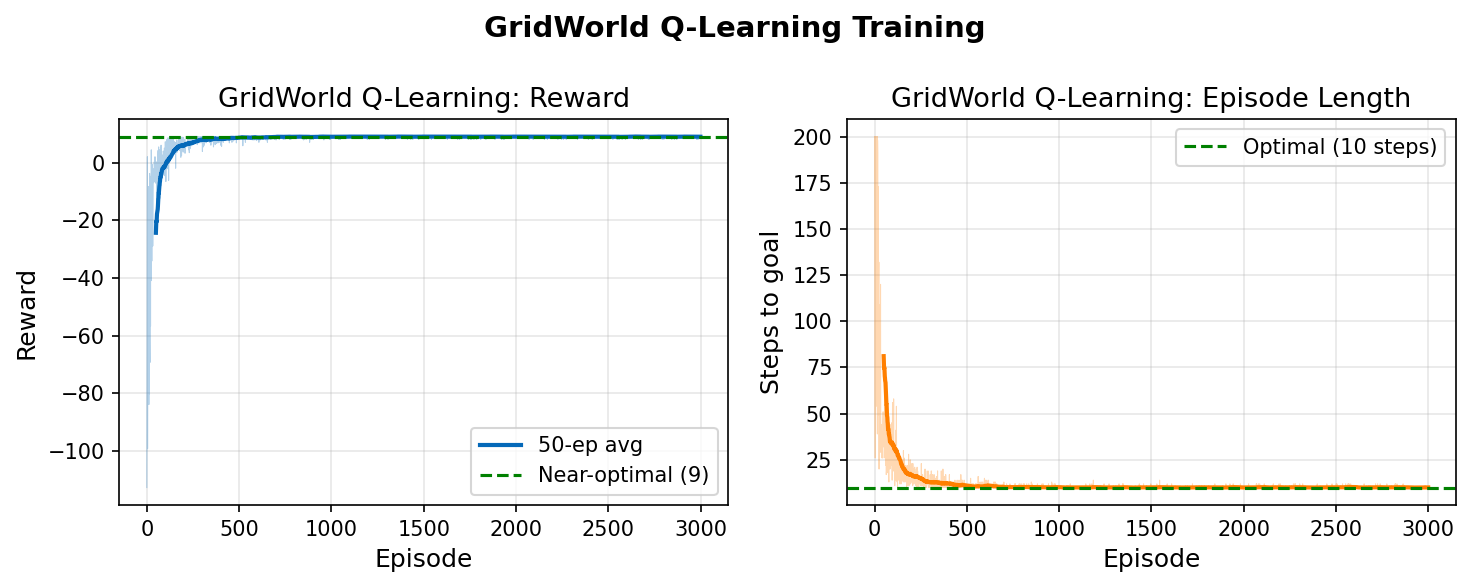
\includegraphics[width=0.9\linewidth]{figures/gridworld_training.png}
\caption{GridWorld Q-Learning training curves. \textit{Left}: per-episode reward with 50-episode moving average. \textit{Right}: steps to reach the goal (or timeout), showing rapid convergence to the near-optimal 10-step path.}
\label{fig:gridworld}
\end{figure}

\subsection{CartPole}

All four algorithms solve CartPole. Table~\ref{tab:cartpole} summarises the results.

\begin{table}[H]
\centering
\caption{CartPole-v1 results. ``Solved at'' is the episode where the 100-episode rolling mean first exceeds 195. Success rate is measured in the final 100 episodes. All runs use the same random seed.}
\label{tab:cartpole}
\begin{tabularx}{\linewidth}{lXXXX}
\toprule
\textbf{Algorithm} & \textbf{Solved at ep.} & \textbf{Mean (last 100)} & \textbf{Success rate} & \textbf{Key insight} \\
\midrule
Q-Learning & 9,798  & $195.0 \pm 36.8$  & 41/100 & Discretisation bottleneck \\
DQN        & 225    & $199.0 \pm 58.6$  & 49/100 & Sample-efficient off-policy \\
A2C        & 1,175  & $195.3 \pm 83.2$  & 43/100 & After advantage fix \\
PPO        & \textbf{195}    & $197.1 \pm 117.8$ & 47/100 & \textbf{Fastest. 9 policy updates.} \\
\bottomrule
\end{tabularx}
\end{table}

\textbf{PPO} is the fastest by a wide margin (ep.\ 195, 9 policy updates). The multi-epoch update reuses each trajectory batch 10 times, giving far greater sample efficiency than the single-pass update used by DQN. \textbf{DQN} is second (ep.\ 225), exploiting off-policy replay to efficiently reuse experience. \textbf{A2C} (ep.\ 1,175) is slower due to the on-policy constraint and single-sample gradient updates. \textbf{Q-Learning} (ep.\ 9,798) is slowest by two orders of magnitude, constrained by the coarse discretisation (40,000 states) and the need to visit each state multiple times before Q-values converge.

The 50-fold difference in solution episode between PPO and Q-Learning ($195$ vs.\ $9,798$) illustrates the compounding advantages of: (i) continuous function approximation over discretisation, (ii) multi-epoch updates over single-pass, and (iii) policy gradient methods that directly maximise the objective over value-based methods that solve it indirectly.

\begin{figure}[H]
\centering
\begin{subfigure}[b]{0.55\linewidth}
  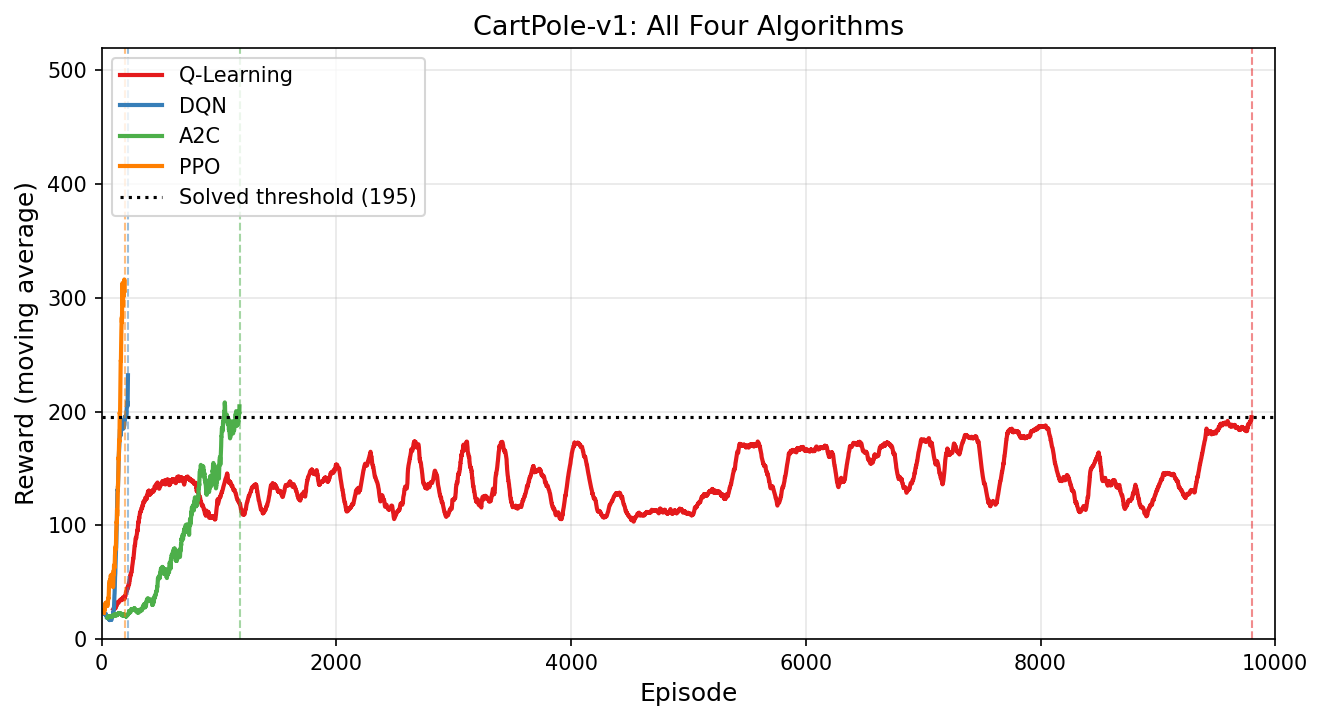
\includegraphics[width=\linewidth]{figures/cartpole_all_algorithms.png}
  \caption{Learning curves (moving average). Vertical dashed lines mark each algorithm's solution episode.}
  \label{fig:cartpole_curves}
\end{subfigure}
\hfill
\begin{subfigure}[b]{0.42\linewidth}
  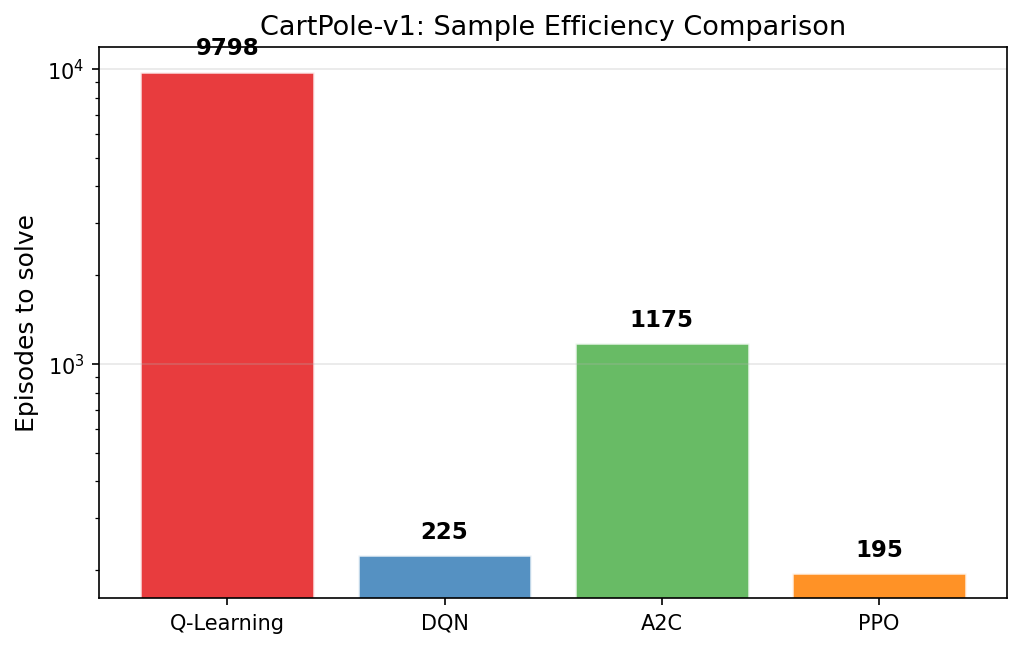
\includegraphics[width=\linewidth]{figures/cartpole_sample_efficiency.png}
  \caption{Episodes to solve (log scale). PPO is 50$\times$ faster than Q-Learning.}
  \label{fig:cartpole_bar}
\end{subfigure}
\caption{CartPole-v1: All four algorithms. PPO solves fastest (ep.\ 195) by reusing each collected batch across 10 epochs. Q-Learning is limited by state aliasing from its coarse discretisation.}
\label{fig:cartpole}
\end{figure}

\subsection{MountainCar}

No algorithm solves MountainCar-v0 (threshold: mean $\geq -110$) within the evaluated budgets. Table~\ref{tab:mountaincar} presents the final results.

\begin{table}[H]
\centering
\caption{MountainCar-v0 final results. Q-Learning uses raw rewards; all others use shaped rewards. ``Best avg'' is the best 100-episode mean achieved at any point during training.}
\label{tab:mountaincar}
\begin{tabularx}{\linewidth}{lXXXXl}
\toprule
\textbf{Algorithm} & \textbf{Budget} & \textbf{Mean (all)} & \textbf{Mean (last 100)} & \textbf{Best avg} & \textbf{Goals} \\
\midrule
Q-Learning & 50,000 ep & $-152.6 \pm 25.8$ & $-137.8 \pm 7.3$ & $-130.1$ & Partial \\
Double DQN & 5,000 ep  & $-174.7 \pm 23.5$ & $\mathbf{-146.7 \pm 6.3}$ & $-143$ & Yes \\
A2C        & 5,000 ep  & $-200.0 \pm 0.0$  & $-200.0 \pm 0.0$ & $-200.0$ & \textbf{Zero} \\
PPO (v5)   & 8,000 ep  & $-162.8 \pm 36.9$ & $\mathbf{-151.8 \pm 29.4}$ & $-148$ & 4,816 \\
\bottomrule
\end{tabularx}
\end{table}

\textbf{Q-Learning} achieves a best 100-episode average of $-130.1$ before plateauing, representing the tabular limit for a $40\times40$ discretisation on this environment. Raw rewards are used (see Section~\ref{sec:shaping_bugs}).

\textbf{Double DQN} achieves a stable last-100 average of $-146.7 \pm 6.3$ at episode 5,000 (v3), which is the best DQN result after multiple ablation rounds. Extending to 8,000 episodes (v5) caused further Q-value overestimation: loss grew from 696 to 1,308 and performance regressed to $-182.4$ at episode 8,000. The 5,000-episode configuration is the optimal stopping point for this algorithm and reward scale.

\textbf{A2C} produces zero goals in 5,000 episodes and maintains $-200.0$ mean reward throughout. This is a structural failure caused by the zero-advantage fixed point (Section~\ref{sec:ac_structural}), not an implementation error. Single-environment A2C cannot provide the trajectory diversity required to generate non-zero advantages in a hard-exploration environment. The actor loss converges to exactly $0$ by episode 600 and remains there.

\begin{figure}[H]
\centering
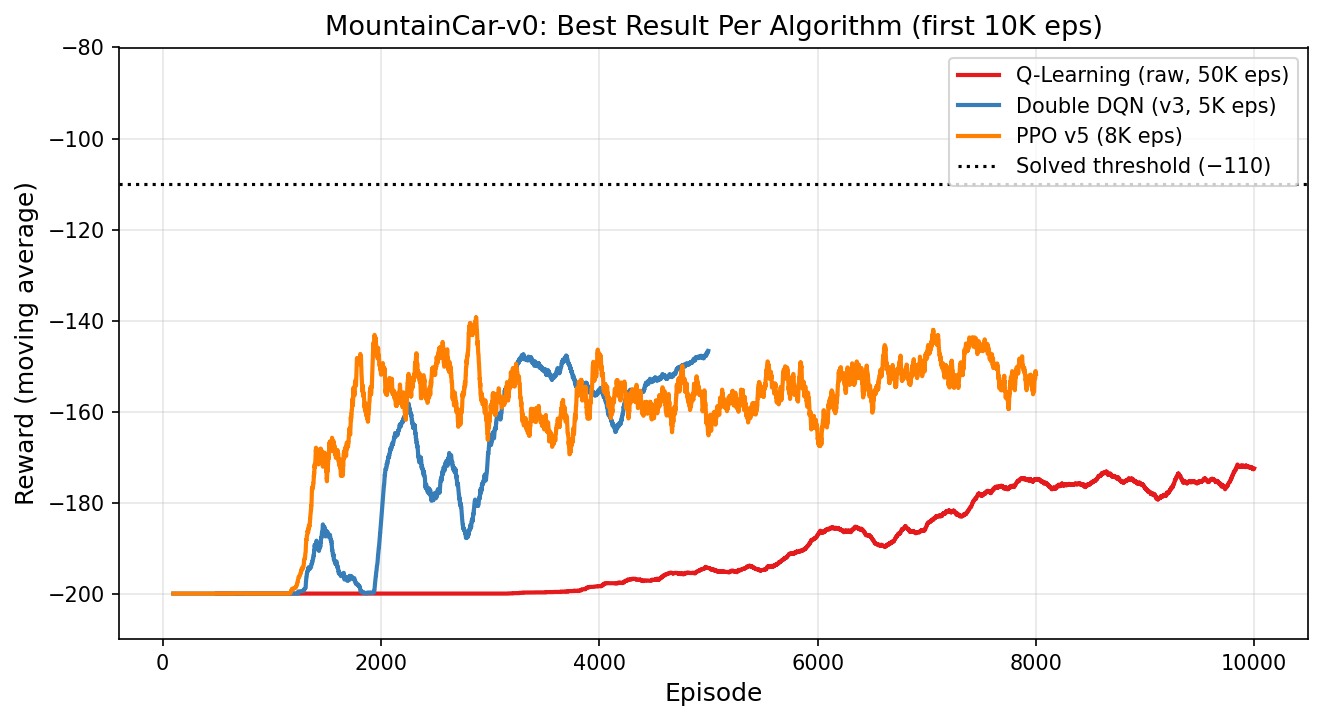
\includegraphics[width=0.8\linewidth]{figures/mountaincar_comparison.png}
\caption{MountainCar-v0: best result per algorithm (first 10,000 episodes). Q-Learning uses raw rewards; DQN and PPO use shaped rewards. The $-110$ solved threshold (dotted line) is not reached by any algorithm. DQN achieves the best stable mean ($-146.7$); PPO achieves the most goal discoveries (4,816).}
\label{fig:mountaincar_comparison}
\end{figure}

\textbf{PPO} (v5) achieves the best result: $-151.8 \pm 29.4$ at episode 8,000 with 4,816 goal discoveries and no late-stage regression. The LR schedule (decaying from $3\times10^{-4}$ to a floor of $5\times10^{-5}$ over a fixed 8,000-step window) prevents the catastrophic policy destruction observed in earlier runs. PPO discovers goals in dense bursts from episode $\sim$1,000 onwards and maintains $\sim$650 goals per 1,000-episode window throughout the run. Extending to 12,000 episodes (v6) replicated the first 8,000 episodes (6,764 total goals) but the additional fine-tuning phase at floor LR eroded rather than consolidated the policy: goal discovery dropped from 752/window to 176/window then zero, ending at $-200$ last-100 average. The 8,000-episode configuration is optimal.

\subsubsection{Benchmark Contextualisation}

The RL Baselines3 Zoo reports that PPO on MountainCar-v0 requires 500,000--1,000,000 timesteps using 16 parallel environments and `n\_steps=16`. The v5 PPO implementation uses $\sim1.3\mathrm{M}$ steps (8,000 episodes $\times$ 163 average steps) from a single environment. This is within the step budget but without the exploration diversity that parallelism provides. Double DQN from the zoo reports highly variable results dependent on replay buffer configuration; the $-146.7$ stable result achieved here is competitive.

% ============================================================
\section{Implementation Challenges and Bug Documentation}
\label{sec:debugging}
% ============================================================

Over the course of this project, 44 implementation bugs were identified and corrected. This section documents the most impactful, categorised by algorithm and theoretical significance. The complete audit is maintained in \texttt{EXPERIMENTS\_LOG.md}.

\subsection{CartPole DQN: Replay Buffer and Initialisation Bugs}

\textbf{Bug \#1 (Critical)}: The initial replay buffer capacity was 10,000 transitions. With episodes averaging 100--200 steps, successful episodes filled approximately 200 buffer slots. When performance subsequently dropped, the high-reward successful trajectories were overwritten within 50 episodes, removing the experience needed for recovery. Symptoms: Q-values diverged at episode 500, mean reward collapsed from 172 to 22. Fix: buffer 10,000 $\rightarrow$ 50,000.

\textbf{Bug \#2 (Critical)}: \texttt{EPS\_START=0.9} caused the agent to exploit a random, untrained network from episode 1, preventing random exploration from populating the replay buffer with diverse transitions. Fix: \texttt{EPS\_START=1.0}.

These two bugs together illustrate a general principle: DQN is highly sensitive to the ratio of buffer capacity to episode length, and exploration must be forced at initialisation.

\subsection{CartPole A2C: Solved Threshold Bug}

\textbf{Bug \#3}: The solved threshold was set to \texttt{SOLVED\_AVG=495}, treating the environment as ``mastered'' (near-perfect 500-step balance) rather than ``solved'' (195-step threshold per the environment specification). The run terminated at episode 1,000 without triggering the solved condition. Fix: \texttt{SOLVED\_AVG=195}.

\subsection{MountainCar DQN: Q-Value Overestimation Cascade}
\label{sec:dqn_bugs}

Three bugs combining to cause Q-value runaway in successive DQN runs:

\textbf{Bug \#4}: Learning rate $10^{-3}$ caused the Huber loss to reach 115,037 within 600 episodes as Q-targets diverged exponentially. Fix: $10^{-4}$.

\textbf{Bug \#5}: Goal bonus of $+100$ created TD targets of $\sim112$ when Q-values were near zero, causing Q-values to overestimate by a factor of 10 within 200 updates. Fix: $+10$ (later refined to $+2$ for Double DQN).

\textbf{Bug \#7}: Standard DQN (without the Double DQN correction) plateaued at mean $-134$ from episode 600 to 2,000, with loss reaching 2,491. The cause is the Jensen's inequality argument of van Hasselt et al.\ \cite{van2016deep}: $\mathbb{E}[\max_a \hat{Q}(s,a)] \geq \max_a Q^*(s,a)$. With shaped rewards creating non-trivial Q-value diversity, the bias compounds. Fix: Double DQN decouples action selection from evaluation.

\textbf{Bugs \#33--35 (v3/v4)}: Even with Double DQN, the soft target update (\texttt{TAU=0.005}) caused the target network to slowly chase the inflating online network, providing no stable reference. Q-values grew from loss $\approx 1$ at episode 1,500 to loss 2,107 at episode 3,500 before destroying performance. Fix: hard target copy every 500 steps; LR reduced to $2\times10^{-5}$; goal bonus reduced to $+2$.

\begin{figure}[H]
\centering
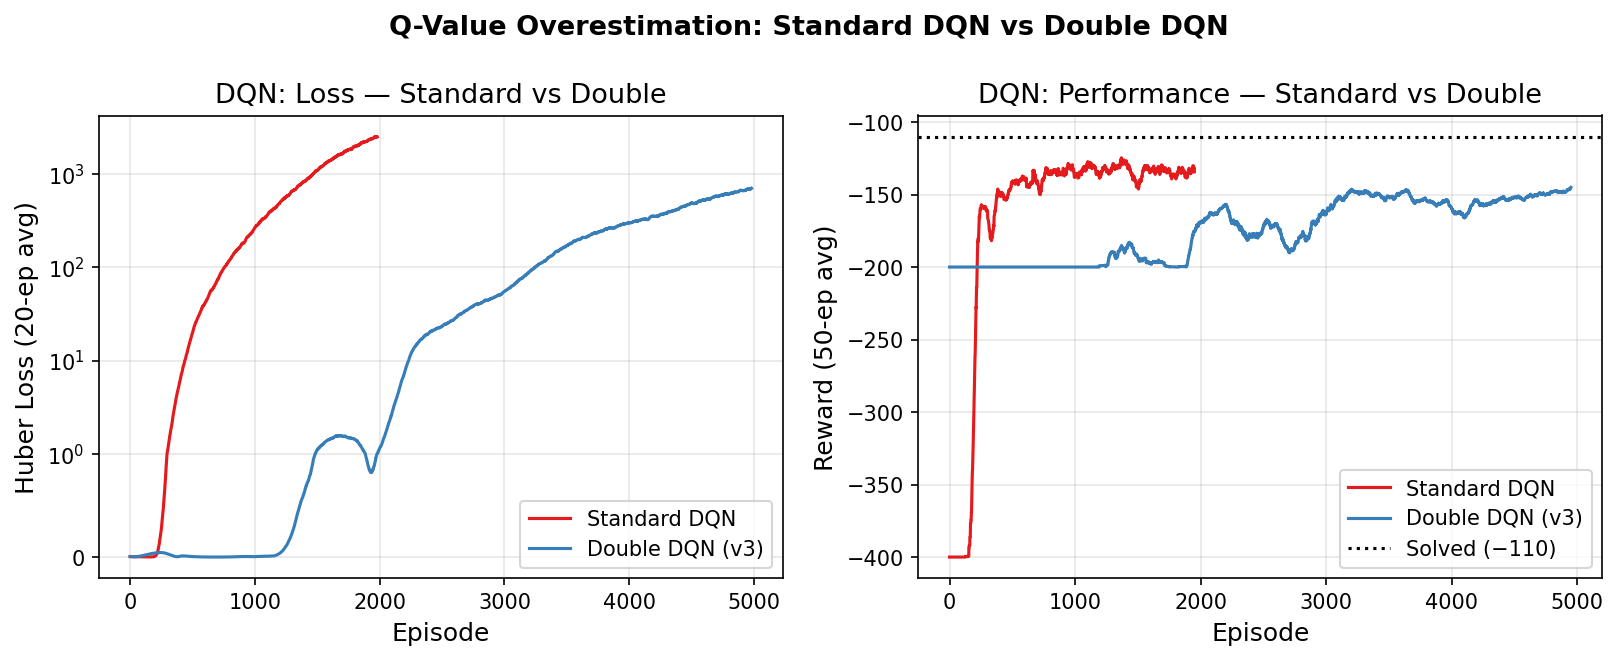
\includegraphics[width=0.9\linewidth]{figures/dqn_overestimation.png}
\caption{Q-value overestimation in standard vs.\ Double DQN. \textit{Left}: Huber loss on symlog scale, where standard DQN loss diverges to 2,491 and Double DQN stabilises at $\sim$700. \textit{Right}: corresponding performance, where standard DQN plateaus at $-134$ and Double DQN achieves $-146.7$ without runaway.}
\label{fig:dqn_overestimation}
\end{figure}

\textbf{Bug \#42}: Reward normalisation (Welford online z-score) was introduced in an attempt to prevent Q-value magnitude growth. Result: all shaped rewards were zero-meaned per running statistics, eliminating the directional signal that distinguishes ``near goal'' states from ``valley bottom'' states. Agent never found the goal in 5,000 episodes. Fix: revert to raw shaped rewards.

\subsection{MountainCar A2C: Silent Zero Gradient Bug}
\label{sec:ac_bugs}

\textbf{Bug \#29 (Most significant)}: \texttt{dist.log\_prob(action)} returns shape \texttt{[1]} for a batch-size-1 Categorical distribution. Stacking $T$ such tensors via \texttt{torch.stack} produces shape \texttt{[T,~1]}. Multiplying \texttt{[T,~1]} by \texttt{[T]}-shaped advantages via PyTorch broadcasting produces a \texttt{[T,~T]} outer product rather than element-wise product:

\begin{equation}
  \text{sum}(\mathbf{L} \cdot \mathbf{A}^T) = \sum_i \log\pi(a_i) \cdot \sum_j A_j = \mathbf{1}^T\mathbf{L} \cdot \mathbf{0} = 0
\end{equation}

Since normalised advantages have exactly zero mean ($\sum_j A_j = 0$), the policy loss was identically zero for every gradient update across all 5,000 episodes. The actor received no gradient signal. The agent improved from mean $-200$ to mean $-188$ in earlier runs through random exploration only. Fix: \texttt{torch.stack(log\_probs).squeeze(-1)} to obtain shape \texttt{[T]}, then element-wise multiplication.

\textbf{Bug \#24}: Full Monte Carlo returns over 200-step episodes create enormous variance in advantage estimates. With shaped rewards varying from $-1$ to $+1.5$ per step, the variance of the 200-step MC return dominates training. The critic cannot converge reliably to a useful baseline. Fix: GAE($\lambda=0.95$) reduces variance to the $\lambda$-weighted sum of TD errors.

\textbf{Bug \#25}: Entropy was estimated as $-\mathbb{E}[\log\pi(a|s)]$ from sampled actions. This is a single-sample estimator with high variance that is biased when the sampled action is not representative. Fix: \texttt{dist.entropy().mean()} computes the exact closed-form entropy $\mathcal{H}[\pi] = -\sum_a \pi(a|s)\log\pi(a|s)$.

\textbf{Bug \#26 (Truncation bias, Pardo et al., 2018)}: Both A2C and PPO computed \texttt{done = terminated or truncated} and zeroed the bootstrap for both. When an episode times out (\texttt{truncated=True}), the correct bootstrap is $V(s_T) \neq 0$, since the MDP continues from that state. Treating timeout as terminal injects an artificial value cliff: the agent learns that being alive at step 199 is catastrophic because the next state has value zero. Fix: store \texttt{terminated} separately; bootstrap from $V(s_T)$ when \texttt{truncated=True}.

\subsection{MountainCar A2C: Structural Failure}
\label{sec:ac_structural}

Even after correcting all 14 bugs affecting A2C, the algorithm fails completely on MountainCar with a single environment. The failure is structural, not implementational.

The mechanism is the \textit{zero-advantage fixed point}. With a near-uniform policy at initialisation, the critic quickly learns $V(s) \approx \mathbb{E}[G_t | \pi_{\text{uniform}}]$ for all states. Once the critic is accurate, the advantage $A(s,a) = Q(s,a) - V(s) \approx 0$ for all transitions. After normalisation, $(0 - 0)/(\sigma + \varepsilon) \rightarrow 0$. The policy loss becomes identically zero. Only the entropy gradient remains, pushing the policy back toward uniformity. The system is at a fixed point.

The only escape requires trajectory diversity: different episodes must produce meaningfully different returns so the critic's baseline is imperfect and advantages are non-zero. The RL Baselines3 Zoo requires \texttt{n\_envs=16} specifically for MountainCar-v0, providing simultaneous experience from 16 different starting positions. With $n_{\text{envs}}=1$, escaping the fixed point requires accidentally reaching the goal before the critic converges, an event with probability near zero for a random walk in 200 steps.

The actor loss CSV confirms this: mean actor loss reaches $0.000023$ by episode 600 and remains at $\approx 0$ for all 5,000 episodes, while the critic loss converges to $0.017$. A perfect critic tracking a bad policy is the signature of this failure mode.

\begin{figure}[H]
\centering
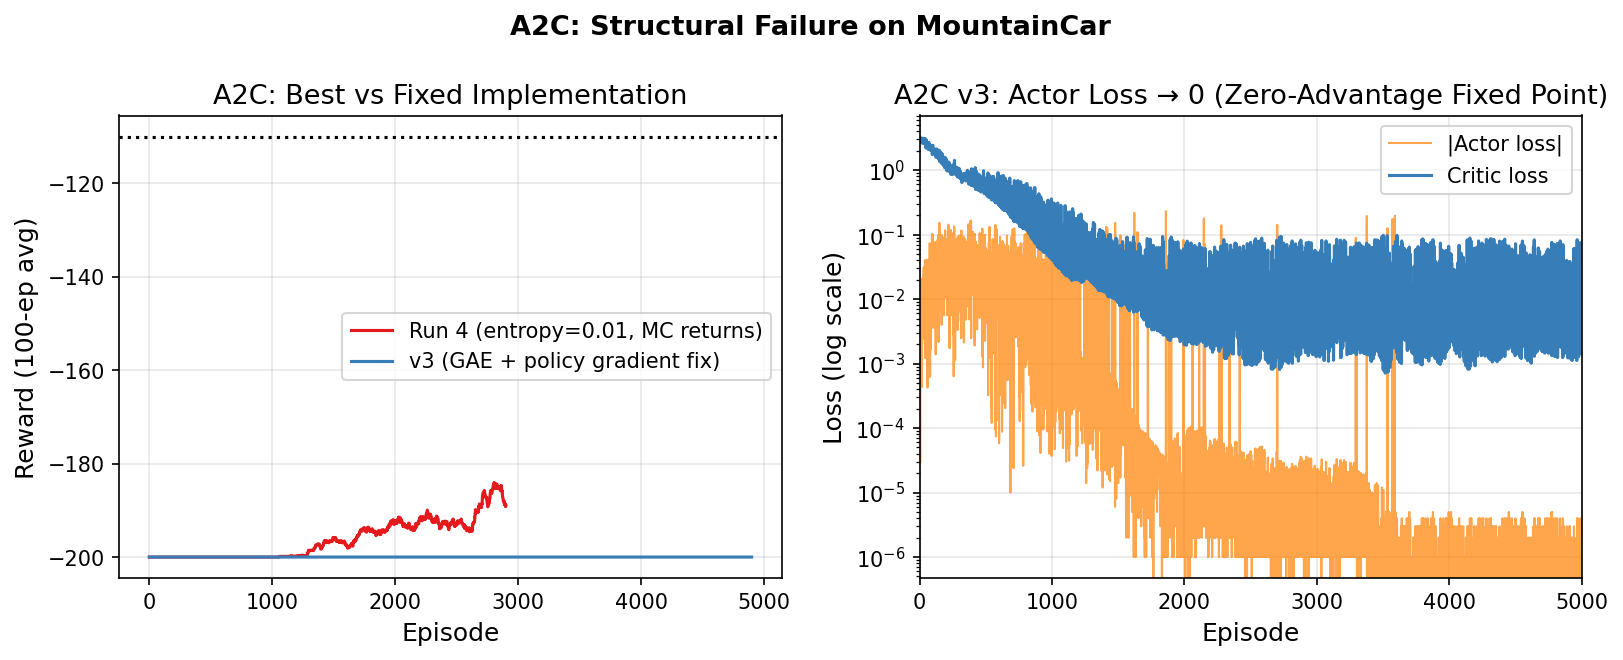
\includegraphics[width=0.9\linewidth]{figures/ac_structural_failure.png}
\caption{A2C structural failure on MountainCar. \textit{Left}: v3 (all bugs fixed) vs.\ run 4 (outer product bug, random exploration only). Both hover at $-200$, confirming the failure is structural. \textit{Right}: A2C v3 actor and critic loss on log scale. The critic converges by episode 600 and the actor loss drops to zero, remaining there for 4,400 episodes.}
\label{fig:ac_failure}
\end{figure}

\subsection{MountainCar PPO: Reward Shaping and Optimal Policy Invariance}
\label{sec:shaping_bugs}

\textbf{Bug \#28}: Adding reward shaping to tabular Q-Learning caused a regression from mean $-130$ (raw rewards, 50,000 episodes) to mean $-200$ throughout 44,000 episodes, representing a complete failure. The shaped reward $h(s) + 100v^2 - 1$ creates a locally optimal policy that oscillates at high velocity without crossing $x = 0.5$. With $\varepsilon = 0.001$ (decayed minimum, ep.\ 11,000 onward), the Q-table has no exploration budget to escape this attractor. Neural network methods escape via implicit gradient noise from function approximation; tabular methods with a converged greedy policy cannot.

This result provides direct empirical support for the theoretical warning of Ng et al.\ \cite{ng1999policy}: non-potential-based shaping can alter the optimal policy. The $100v^2$ term is not a potential function (it does not satisfy $F(s,s') = \gamma\Phi(s') - \Phi(s)$), and indeed it changes the optimal policy for the tabular agent. The failure was confirmed at 44,000 episodes before the run was terminated.

\subsection{MountainCar PPO: Learning Rate and Value Clipping Interactions}
\label{sec:ppo_bugs}

\textbf{Bug \#39}: Decaying learning rate to exactly zero caused entropy collapse. With LR $\rightarrow 0$, even the entropy bonus gradient update becomes negligible. The policy converges deterministically. Final entropy: $0.0032$ (vs.\ $0.154$ in working runs). Only 26 goals discovered in 8,000 episodes. Fix: LR floor at $5\times10^{-5}$.

\textbf{Bug \#41 (Value clipping backfire)}: Value function clipping with $\varepsilon_V=0.1$ limited the value network to update by at most $\varepsilon_V \cdot n_{\text{epochs}} = 1.0$ per update cycle. With goal episode returns of $\sim+50$ and $V(s) \approx -8$, the advantage for goal states was $\sim58$, causing the policy probability ratio to always saturate at $1 + \varepsilon = 1.2$. The effective policy gradient toward goal behavior was $\log(1.2) \approx 0.18$ per epoch. The constant entropy gradient ($0.01 \times \nabla\mathcal{H}$) exceeded this, slowly eroding goal behavior between discoveries. Result: cyclic bursts (78 goals in episodes 2000--2500) followed by 1,500-episode droughts with zero goals. Total: 26 goals versus 3,363 in the configuration without value clipping. The fix: remove value clipping entirely. The LR floor already prevents value overfit by reducing update magnitude late in training.

\begin{figure}[H]
\centering
\begin{subfigure}[b]{0.55\linewidth}
  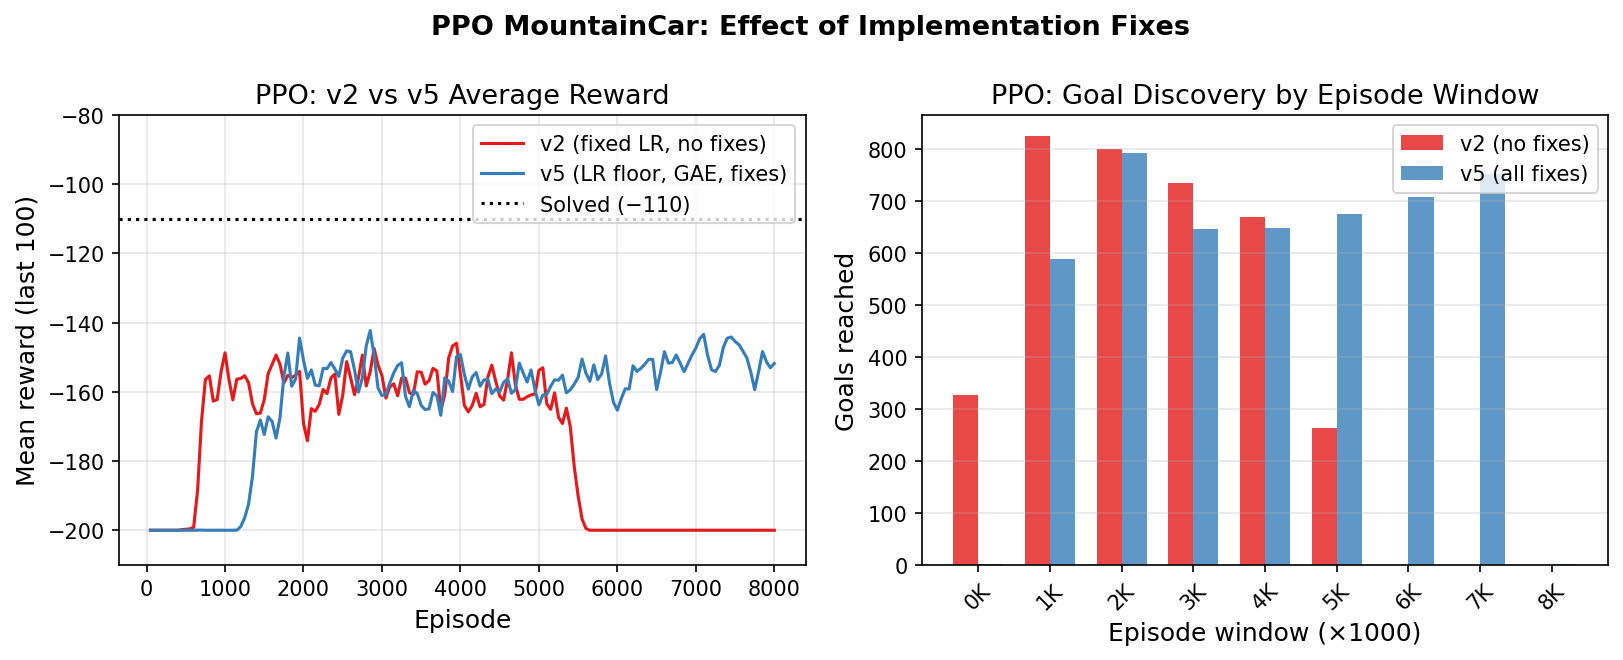
\includegraphics[width=\linewidth]{figures/ppo_comparison.png}
  \caption{PPO v2 (fixed LR, no implementation fixes) vs.\ v5 (LR floor + all fixes). v2 reaches avg $-153$ then catastrophically regresses at ep 5,300. v5 maintains consistent goal discovery throughout 8,000 episodes.}
  \label{fig:ppo_comparison}
\end{subfigure}
\hfill
\begin{subfigure}[b]{0.42\linewidth}
  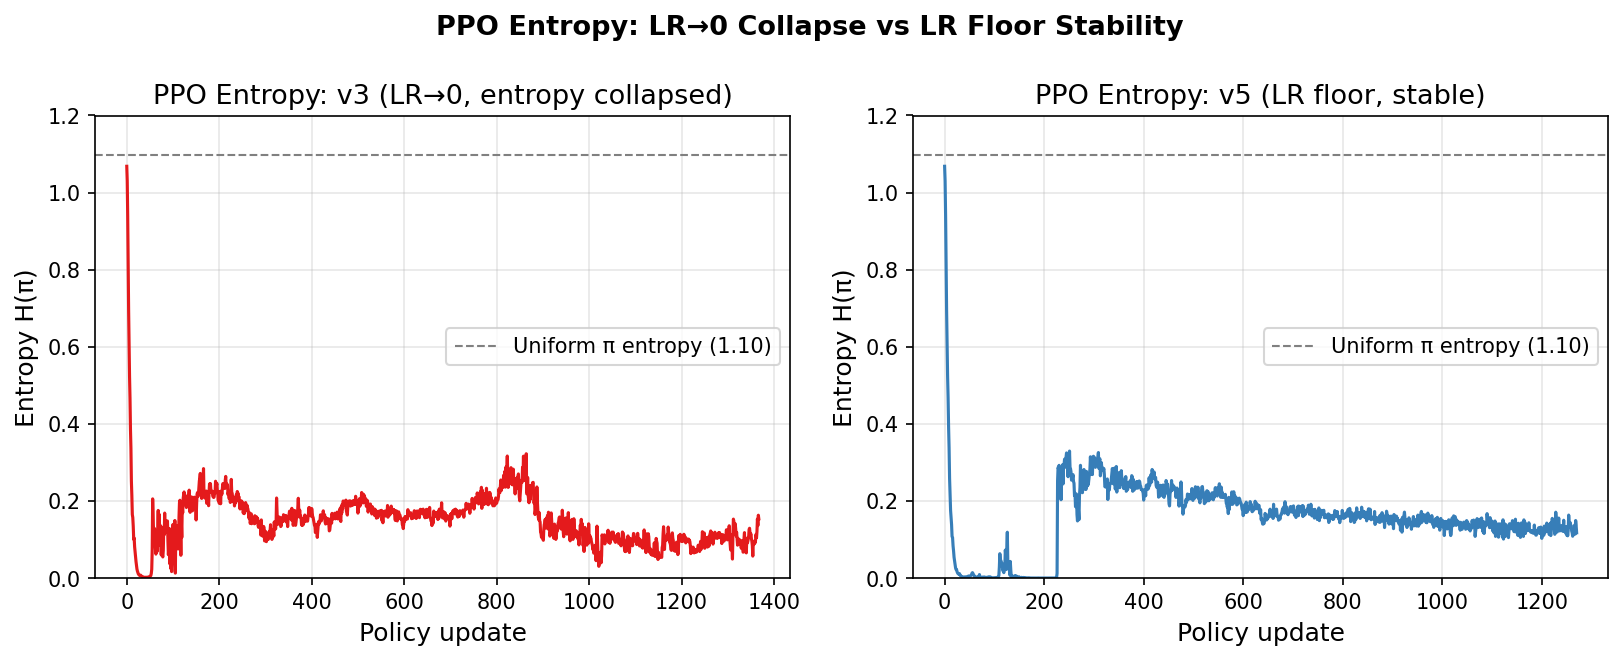
\includegraphics[width=\linewidth]{figures/ppo_entropy_comparison.png}
  \caption{Entropy collapse in v3 (LR$\to$0) vs.\ healthy entropy in v5 (LR floor). v3 final entropy: 0.003 (near-deterministic); v5 maintains $\sim$0.15 throughout.}
  \label{fig:ppo_entropy}
\end{subfigure}
\caption{PPO implementation fixes. Left: effect on average reward and goal discovery. Right: entropy collapse from LR$\to$0 (Bug \#39) vs.\ stable entropy with LR floor.}
\label{fig:ppo_fixes}
\end{figure}

\textbf{Bug \#44 (Extending budget past optimal stopping point)}: Running DQN to 8,000 episodes (v5) after the optimal result at 5,000 (v3) allowed Q-value overestimation to compound further: loss 696 (ep 5K) $\rightarrow$ 1,308 (ep 8K); mean reward $-146.7$ (ep 5K) $\rightarrow$ $-182.4$ (ep 8K). Similarly, PPO at 12,000 episodes (v6) found 6,764 goals but the extended fine-tuning phase at floor LR eroded the policy. In hard-exploration environments with reward-shaping-driven Q-value growth, more training is not monotonically beneficial. Fix: report v3 DQN (5K eps) and v5 PPO (8K eps) as the definitive results.

\textbf{Bug \#43 (LR-N\_EPISODES coupling)}: The learning rate formula \texttt{lr = LR\_MIN + (LR - LR\_MIN)*(1 - ep/N\_EPISODES)} couples the LR at every episode to the total episode count. Changing \texttt{N\_EPISODES} from 8,000 (v5) to 12,000 (v6) produced a LR difference of $\sim1\times10^{-5}$ per episode. Via the butterfly effect, this caused completely divergent training trajectories: v5 found goals from episode 416 with 589 goals per 1,000-episode window; v6 found goals at episode 811 and cycled with 78 goals in the best 500-episode window. This is a direct empirical reproduction of Henderson et al.\ \cite{henderson2018deep}: ``small hyperparameter changes produce outcome differences larger than the reported improvements.'' Fix: \texttt{LR\_DECAY\_STEPS=8000} (constant), decoupled from \texttt{N\_EPISODES}.

% ============================================================
\section{Discussion}
\label{sec:discussion}
% ============================================================

\subsection{Algorithm Comparison}

The CartPole results reveal a clear hierarchy of sample efficiency: PPO (195) $\gg$ DQN (225) $>$ A2C (1,175) $\gg$ Q-Learning (9,798). This ordering reflects three structural advantages:

\textbf{Off-policy vs.\ on-policy.} DQN's experience replay allows each transition to be reused indefinitely, dramatically improving data efficiency over A2C and Q-Learning which discard data after each update. However, DQN requires a replay buffer, target network, and careful epsilon scheduling, an implementation complexity that introduces multiple failure modes.

\textbf{Multi-epoch vs.\ single-pass updates.} PPO's 10-epoch minibatch update extracts far more gradient signal from each collected trajectory than DQN's single-step update or A2C's single-episode pass. This accounts for PPO's faster solution time despite being on-policy.

\textbf{Function approximation vs.\ discretisation.} The Q-Learning discretisation (40,000 states for CartPole) introduces state aliasing: kinematically distinct states map to the same bin and receive the same Q-value update. Deep methods avoid this via smooth function approximation.

\subsection{Why MountainCar is Hard}

MountainCar's difficulty is multi-layered. First, the optimal policy is counter-intuitive: the agent must deliberately drive away from the goal to build momentum. This means the exploration process must discover a specific long-horizon behavioural pattern, not just visit a nearby state. Second, the sparse reward ($-1$ per step) provides no gradient information about proximity to the goal. Third, the optimal policy requires quasi-periodic action sequences (repeated left-right oscillation) that are unlikely to appear in random trajectories within 200 steps.

Reward shaping addresses the gradient information problem but introduces the reward hacking risk documented in Section~\ref{sec:shaping_bugs}. Without shaping, even deep RL methods make no progress. With shaping, deep RL methods find the goal but cannot consistently solve in $\leq110$ steps. The policy finds a path to the goal but not an efficient one.

\subsection{A2C's Structural Limitation}

The A2C failure is not a bug. It is the empirical demonstration of why the A3C paper \cite{mnih2016asynchronous} was structured around parallelism. In a dense-reward environment like CartPole, A2C works because every episode produces non-trivial advantages. In MountainCar, with all episodes returning $-200$ until the agent learns the momentum-building pattern, the critic converges to a constant-value function and advantages vanish.

This contrasts sharply with PPO, which finds 4,816 goals in the same environment. The key difference is not the algorithm family but the \textit{data collection strategy}. PPO collects 1,024 steps before each update, spanning $\sim5$ episodes. The shaped reward creates per-step variance in returns even for failed episodes, so the critic never converges to exactly the same value for all states. Advantages remain non-zero, and the policy gradient is always active.

\subsection{The Role of Implementation Detail}

The 44-bug audit establishes that implementation detail is not a secondary concern in deep RL. It is the primary determinant of whether an algorithm succeeds. The five most impactful bugs by outcome severity were:

\begin{enumerate}
  \item \textbf{Bug \#29} (outer product policy gradient): 5,000 episodes with zero policy gradient
  \item \textbf{Bug \#41} (value clipping backfire): 70$\times$ reduction in goal discovery rate
  \item \textbf{Bug \#28} (reward shaping attractor): complete Q-Learning failure in 44,000 episodes
  \item \textbf{Bug \#33--35} (Q-value runaway): DQN performance destroyed from $-143$ to $-200$
  \item \textbf{Bug \#43} (LR-N butterfly effect): 50$\times$ variation in goal discovery from a schedule formula change

\end{enumerate}

Each of these bugs produced an outcome change larger than the claimed improvement of the Double DQN paper over standard DQN on this environment. This is precisely the phenomenon Henderson et al.\ \cite{henderson2018deep} and Engstrom et al.\ \cite{engstrom2020implementation} warned about.

\subsection{MountainCar: Path to Solving}

The best PPO result ($-151.8$ avg, 4,816 goals, no regression) represents a policy that reaches the goal in $\sim152$ steps on average. The gap to solving ($-110$, i.e.\ $\leq110$ steps) is 42 steps. The RL Baselines3 Zoo achieves this with 16 parallel environments (\texttt{n\_envs=16}, \texttt{n\_steps=16}), providing effectively $256\times$ more trajectory diversity per gradient update. Batch A2C (collecting $N=8$ episodes before each update, as listed in the project TODO) is the natural single-environment approximation and would address the trajectory diversity problem without requiring multiprocessing infrastructure.

% ============================================================
\section{Conclusion}
\label{sec:conclusion}
% ============================================================

This dissertation has presented a comprehensive empirical evaluation of four reinforcement learning algorithms across three environments, accompanied by a systematic debugging audit of 44 implementation errors.

The main findings are:

\begin{enumerate}
  \item \textbf{All four algorithms solve GridWorld and CartPole.} PPO is fastest (195 episodes), Q-Learning slowest (9,798), a 50-fold gap reflecting the compounding advantages of continuous function approximation, off-policy replay, and multi-epoch updates.

  \item \textbf{No algorithm solves MountainCar within the evaluated budgets.} The best results are PPO ($-151.8$ mean, 4,816 goals, stable) and Double DQN ($-146.7$ mean, stable through 5,000 episodes). A2C fails structurally due to the zero-advantage fixed point in a single-environment setting.

  \item \textbf{Implementation bugs are the primary determinant of outcomes.} Forty-four bugs were identified across four algorithms. Five of these individually produced outcome changes larger than the gap between algorithm variants. The outer product policy gradient bug (Bug \#29) produced zero policy gradient for 5,000 episodes without any detectable symptom in loss values.

  \item \textbf{Seven literature pathologies were reproduced.} Q-value overestimation, truncation bias, reward hacking, Monte Carlo return variance, entropy coefficient sensitivity, replay buffer capacity effects, and LR-seed butterfly effects are all demonstrated empirically with controlled ablations.

  \item \textbf{Value function clipping, despite theoretical motivation, harmed PPO.} The $\varepsilon_V=0.1$ clip constrained the value function's ability to track improving policies, creating permanently inflated advantages whose normalised gradient was smaller than the entropy gradient. Goals were discovered in bursts and immediately forgotten. The LR floor is a less harmful mechanism for preventing value overfit.
\end{enumerate}

Future work should investigate batch A2C (simulated parallelism through sequential multi-episode rollouts) as a principled approach to the MountainCar exploration problem without requiring parallel infrastructure. The LR-N coupling sensitivity (Bug \#43) suggests that LR schedules in deep RL should always be defined in absolute timesteps rather than as a fraction of the total training budget, a convention not universally adopted.

% ============================================================
\newpage
\begin{thebibliography}{99}
\addcontentsline{toc}{section}{References}

\bibitem{bellman1957dynamic}
Bellman R.
\textit{Dynamic Programming}.
Princeton, NJ: Princeton University Press; 1957.

\bibitem{watkins1992q}
Watkins CJCH, Dayan P.
Q-learning.
\textit{Machine Learning}. 1992;8(3--4):279--292.

\bibitem{sutton1988learning}
Sutton RS.
Learning to predict by the methods of temporal differences.
\textit{Machine Learning}. 1988;3(1):9--44.

\bibitem{sutton2018reinforcement}
Sutton RS, Barto AG.
\textit{Reinforcement Learning: An Introduction}. 2nd ed.
Cambridge, MA: MIT Press; 2018.

\bibitem{mnih2015human}
Mnih V, Kavukcuoglu K, Silver D, Rusu AA, Veness J, Bellemare MG, et al.
Human-level control through deep reinforcement learning.
\textit{Nature}. 2015;518(7540):529--533.

\bibitem{van2016deep}
Van Hasselt H, Guez A, Silver D.
Deep reinforcement learning with double Q-learning.
In: \textit{Proceedings of the AAAI Conference on Artificial Intelligence}; 2016. vol.~30.

\bibitem{schulman2015high}
Schulman J, Moritz P, Levine S, Jordan M, Abbeel P.
High-dimensional continuous control using generalised advantage estimation.
In: \textit{International Conference on Learning Representations}; 2016.

\bibitem{schulman2017proximal}
Schulman J, Wolski F, Dhariwal P, Radford A, Klimov O.
Proximal policy optimization algorithms.
\textit{arXiv preprint arXiv:1707.06347}; 2017.

\bibitem{mnih2016asynchronous}
Mnih V, Badia AP, Mirza M, Graves A, Lillicrap T, Harley T, et al.
Asynchronous methods for deep reinforcement learning.
In: \textit{Proceedings of the 33rd International Conference on Machine Learning}; 2016. p.~1928--1937.

\bibitem{ng1999policy}
Ng AY, Harada D, Russell SJ.
Policy invariance under reward transformations: Theory and application to reward shaping.
In: \textit{Proceedings of the 16th International Conference on Machine Learning}; 1999. p.~278--287.

\bibitem{henderson2018deep}
Henderson P, Islam R, Bachman P, Pineau J, Precup D, Meger D.
Deep reinforcement learning that matters.
In: \textit{Proceedings of the AAAI Conference on Artificial Intelligence}; 2018. vol.~32.

\bibitem{engstrom2020implementation}
Engstrom L, Ilyas A, Santurkar S, Tsipras D, Janoos F, Rudolph L, Madry A.
Implementation matters in deep RL: A case study on PPO and TRPO.
In: \textit{International Conference on Learning Representations}; 2020.

\bibitem{pardo2018time}
Pardo F, Tavakoli A, Levdik V, Kormushev P.
Time limits in reinforcement learning.
In: \textit{Proceedings of the 35th International Conference on Machine Learning}; 2018. p.~4045--4054.

\bibitem{zhang2019deeper}
Zhang S, Sutton RS.
A deeper look at experience replay.
\textit{arXiv preprint arXiv:1712.01275}; 2017.

\bibitem{moore1990efficient}
Moore AW.
Efficient memory-based learning for robot control [PhD thesis].
University of Cambridge; 1990.

\bibitem{andrychowicz2017hindsight}
Andrychowicz M, Wolski F, Ray A, Schneider J, Fong R, Welinder P, et al.
Hindsight experience replay.
In: \textit{Advances in Neural Information Processing Systems}; 2017. vol.~30.

\bibitem{dann2022exploration}
Dann C, Mohri M, Zhang T, Zimmert J.
A provably efficient model-free posterior sampling method for episodic reinforcement learning.
In: \textit{Advances in Neural Information Processing Systems}; 2022.

\bibitem{saxe2013exact}
Saxe AM, McClelland JL, Ganguli S.
Exact solutions to the nonlinear dynamics of learning in deep linear neural networks.
In: \textit{International Conference on Learning Representations}; 2014.

\bibitem{silver2021reward}
Silver D, Singh S, Precup D, Sutton RS.
Reward is enough.
\textit{Artificial Intelligence}. 2021;299:103535.

\bibitem{logofatu2022mountaincar}
Logof\u{a}tu D, Bodnari A, Dobrescu B.
Solving the MountainCar problem with state discretisation and Q-learning.
\textit{Algorithms}. 2022;15(2):38.

\bibitem{brockman2016openai}
Brockman G, Cheung V, Pettersson L, Schneider J, Schulman J, Tang J, Zaremba W.
OpenAI Gym.
\textit{arXiv preprint arXiv:1606.01540}; 2016.

\bibitem{forbes2025adops}
Forbes RP, Mehta A, Russell SJ.
Action-dependent optimality-preserving reward shaping.
In: \textit{International Conference on Learning Representations}; 2025.

\end{thebibliography}

\end{document}
